\chapter{\ifenglish Background Knowledge and Theory\else ทฤษฎีที่เกี่ยวข้อง\fi}

\qquad การทำโครงงาน เริ่มต้นด้วยการศึกษาค้นคว้า ทฤษฎีที่เกี่ยวข้อง หรือ งานวิจัย/โครงงาน ที่เคยมีผู้นำเสนอไว้แล้ว
ซึ่งเนื้อหาในบทนี้ก็จะเกี่ยวกับการอธิบายถึงสิ่งที่เกี่ยวข้องกับโครงงาน เพื่อให้ผู้อ่านเข้าใจเนื้อหาในบทถัดๆ ไปได้ง่ายขึ้น

\section{แพลตฟอร์มที่คล้ายคลึงกัน}
  \subsection{GradeScope}
    \begin{figure}[!h]
      \centering
      
\includegraphics[width=0.6\textwidth]{image/Background/gradescope-logo.png}
      \caption[GradeScope]{GradeScope logo}
      \label{fig:gradescope_pic}
    \end{figure}
    \FloatBarrier
    \qquad GradeScope เป็นแพลตฟอร์มหนึ่งที่ออกแบบมาเพื่อช่วยแก้ปัญหาการตรวจและให้คะแนนใบงาน ข้อสอบ หรือการบ้านของนักศึกษา
    ให้เป็นไปอย่างมีประสิทธิภาพมากยิ่งขึ้น สามารถรองรับกระบวนการสอนที่มีใบงานในรูปแบบกระดาษหรือไฟล์ดิจิทัล โดยมีการแสดงผล
    ที่เป็นมิตรกับผู้ใช้ และสามารถเข้าถึงได้ผ่านอินเทอร์เน็ต แพลตฟอร์ม GradeScope มีฟังก์ชันหลักดังนี้
      \begin{enumerate}
        \item การอัปโหลดและกำหนดเกณฑ์สำหรับการตรวจใบงาน ผู้สอนสามารถอัปโหลดใบงานและข้อสอบเป็นรูปภาพหรือไฟล์ (PDF) และกำหนดเกณฑ์การให้คะแนน (Rubrics) ได้อย่างยืดหยุ่นตามความต้องการ
        \item การตรวจและให้คะแนนที่สะดวกสบาย ระบบ GradeScope ช่วยให้ผู้สอนสามารถตรวจและให้คะแนนใบงานได้อย่างรวดเร็วผ่านหน้าจอเดียว ซึ่งผู้สอนสามารถใส่คะแนนและความคิดเห็นได้ในที่เดียวกัน และปรับคะแนนหากมีการเปลี่ยนแปลงเกณฑ์การให้คะแนน
        \item การแสดงผลและวิเคราะห์คะแนน GradeScope มีระบบการแสดงผลคะแนนของนักศึกษาในรูปแบบกราฟและสถิติต่างๆ เพื่อช่วยให้ผู้สอนวิเคราะห์ผลการเรียนรู้ของนักศึกษาในกระบวนวิชาได้ง่ายขึ้น
        \item ความสะดวกในการค้นหาและการจัดเก็บข้อมูล ระบบ GradeScope ช่วยให้ผู้สอนสามารถค้นหาใบงานและข้อสอบได้ง่ายและรวดเร็ว ไม่ต้องกังวลเรื่องการสูญหายของกระดาษ และมีการจัดเก็บข้อมูลที่เป็นระบบ
      \end{enumerate}
  \subsection{Mango}
    \begin{figure}[!h]
      \centering
      
\includegraphics[width=0.4\textwidth]{image/Background/Mango-cmu.png}
      \caption[Mango]{Mango logo}
      \label{fig:mango_pic}
    \end{figure}
    \FloatBarrier
    \qquad MangoCanvas เป็นระบบ LMS ของมหาวิทยาลัยเชียงใหม่ ที่ออกแบบมาเพื่อช่วยอาจารย์ในการจัดการการเรียนการสอน โดยผู้สอนสามารถเพิ่มกระบวนวิชาและจัดการเนื้อหา เช่น การบ้านและแบบฝึกหัด รวมถึงประกาศคะแนนและติดตามความก้าวหน้าของนักศึกษาได้ ระบบมีการรองรับการนำเข้าคะแนนในรูปแบบสเปรดชีต ซึ่งสามารถใช้แม่แบบที่ระบบเตรียมไว้ให้ หลังจากที่นำเข้าคะแนน ระบบจะคำนวณค่าทางสถิติให้อัตโนมัติ และหากผู้สอนต้องการแก้ไขคะแนน สามารถทำได้ในระบบโดยไม่ต้องกลับไปแก้ในสเปรดชีต
  \subsection{MS Team}
    \begin{figure}[!h]
      \centering
      
\includegraphics[width=0.6\textwidth]{image/Background/Microsoft-Teams-Logo.png}
      \caption[Microsoft Teams]{Microsoft Teams logo}
      \label{fig:microsoft_teams_pic}
    \end{figure}
    \FloatBarrier
    \qquad Microsoft Teams เป็นแอพลิเคชั่นที่มีความหลากหลายและมีความยืดหยุ่น ช่วยให้การจัดการการเรียนการสอนออนไลน์ และการทำงานเป็นทีมเป็นไปอย่างมีประสิทธิภาพ ช่วยเพิ่มความสะดวกให้กับผู้สอนในการสื่อสาร การมอบหมายงาน และการจัดเก็บข้อมูลต่างๆ ได้ในแพลตฟอร์มเดียว

\section{User Experience and User Interface}
  \qquad UX/UI คือการออกแบบผลิตภัณฑ์ดิจิทัล เช่น เว็บไซต์หรือแอปพลิเคชัน
  โดยที่ UX (User Experience) คือประสบการณ์ของผู้ใช้โดยรวม เน้นความรู้สึกและการใช้งานที่ง่ายและมีประสิทธิภาพ
  ส่วน UI (User Interface) คือส่วนที่ผู้ใช้มองเห็นและโต้ตอบด้วย เช่น ปุ่ม, สี, และการจัดวาง เพื่อให้ผลิตภัณฑ์นั้นดูสวยงามและน่าใช้
  \subsection{User-Centered Design (UCD)}
    \begin{figure}[h!]
      \begin{center}
        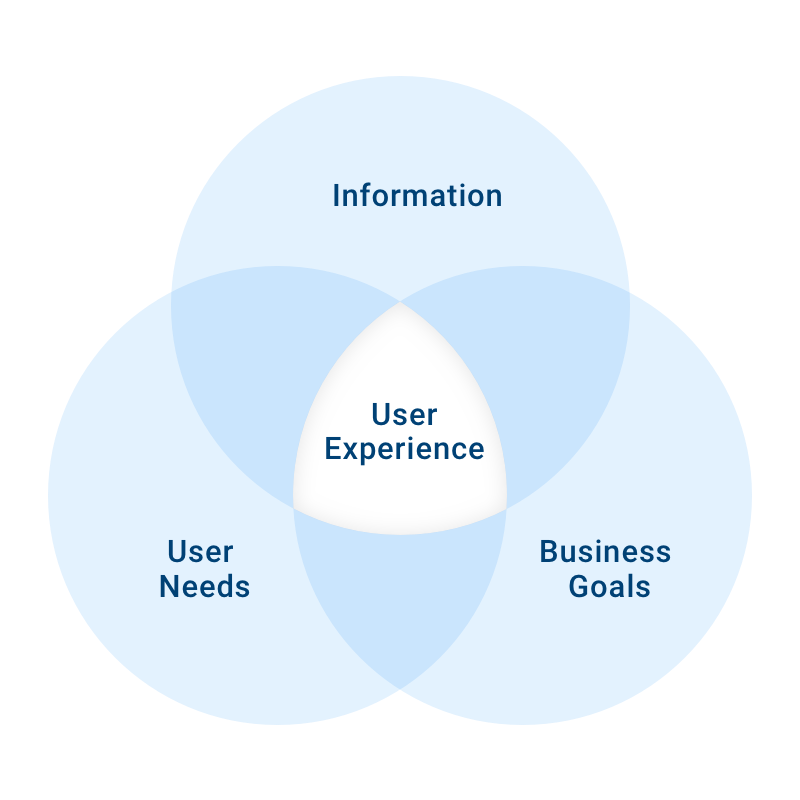
\includegraphics[scale=0.25]{image/Background/UDC.png}
      \end{center}
      \caption[User-Centered Design]{How to design in User-Centered Way}
      \label{fig:udc_pic}
    \end{figure}
    \FloatBarrier
    \qquad เป็นหลักการการออกแบบที่จัดระดับความสําคัญของความต้องการและความชอบของผู้ใช้งานตลอดกระบวนการออกแบบ โดยการทําความเข้าใจผู้ใช้เป้าหมายและบริบทของผู้ใช้ เพื่อสร้างเว็บแอพพลิเคชั่นที่ใช้งาน ง่ายมีประสิทธิภาพในการใช้งานโดยทั่วไปหลักการนี้จะเกี่ยวข้องกับการออกแบบซํ้าๆเช่น การวิจัยผู้ใช้ การสร้างต้นแบบ และการทดสอบการใช้งานเพื่อปรับปรุงประสบการณ์ของผู้ใช้อย่างต่อเนื่อง \cite{UCD1}\cite{UCD2}

  \subsection{Jakob’s Law}
    \qquad เป็นหลักการการออกแบบว่าด้วยการพัฒนาหรือปรับปรุงผลิตภัณฑ์ไม่ว่าจะเป็นสิ่งของ หรือบนเว็บไซต์
    แอพพลิเคชั่นจากความคุ้นเคยเดิมของผู้ใช้ ให้สามารถใช้งานผลิตภัณฑ์ได้ง่ายและสะดวกมากขึ้นโดยที่ไม่ต้องเริ่ม
    เรียนรู้การใช้งานใหม่อีกครั้ง โดยจะใช้รูปแบบ UI ที่ผู้ใช้คุ้นเคยเพื่อไม่ให้ผู้ใช้ต้องปรับตัวใหม่หรือการจัดองค์ประกอบของส่วนต่างๆ
    ในหน้า layout ให้เหมาะสม ไม่พยายามเปลี่ยนแปลงประสบการณ์ของผู้ใช้มากจนเกินไป ซึ่งความสอดคล้องตรงนี้จะช่วยให้
    ผู้ใช้รู้สึกสบายและมั่นใจในการใช้ผลิตภัณฑ์มากขึ้น เมื่อองค์ประกอบบนเว็บไซต์ต้องทํางานสอดคล้องกับความคาดหวังของผู้ใช้งาน \cite{Jakob}

\section{Platform Development}
  \subsection{Sprints}
    \begin{figure}[!ht]
      \centering
      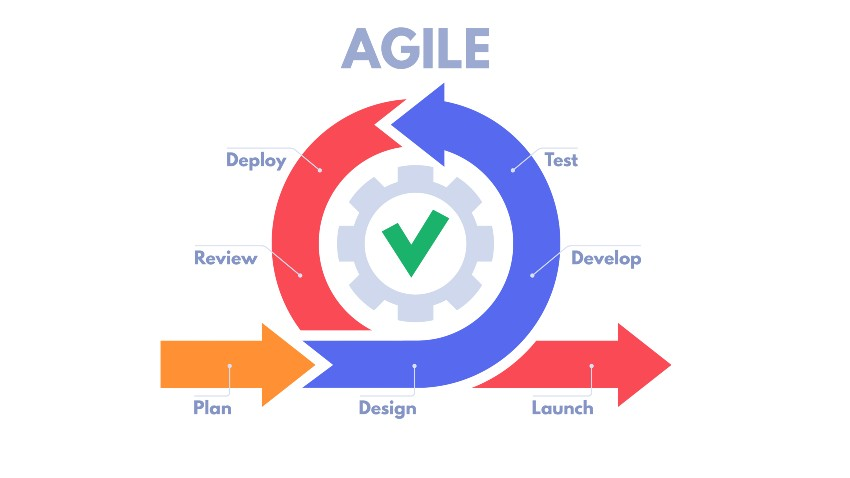
\includegraphics[width=0.8\textwidth]{image/Background/Sprints.jpg}
      \caption[Sprints]{Sprints concept}
      \label{fig:sprints_pic}
    \end{figure}
    \FloatBarrier
    \qquad Sprints คือ ช่วงเวลาที่กำหนดไว้ล่วงหน้าในกระบวนการพัฒนาซอฟต์แวร์แบบ Agile
    ซึ่งทีมพัฒนาจะทำงานร่วมกันเพื่อสร้างและส่งมอบฟีเจอร์ หรือส่วนประกอบของซอฟต์แวร์ในระยะเวลาที่กำหนด
    โดยที่ทั่วไป Sprints จะมีระยะเวลาประมาณ 1-4 สัปดาห์ ซึ่งในแต่ละ Sprint ทีมจะวางแผนงาน
    พัฒนา ทดสอบ และส่งมอบซอฟต์แวร์ที่มีคุณภาพสูงให้กับผู้ใช้หรือลูกค้าได้อย่างต่อเนื่อง
    การใช้ Sprints ช่วยให้ทีมสามารถปรับตัวและตอบสนองต่อการเปลี่ยนแปลงได้อย่างรวดเร็ว
    และส่งมอบซอฟต์แวร์ที่ตรงกับความต้องการของผู้ใช้มากยิ่งขึ้น \cite{Sprint}
  \subsection{Agile}
    \begin{figure}[!ht]
      \centering
      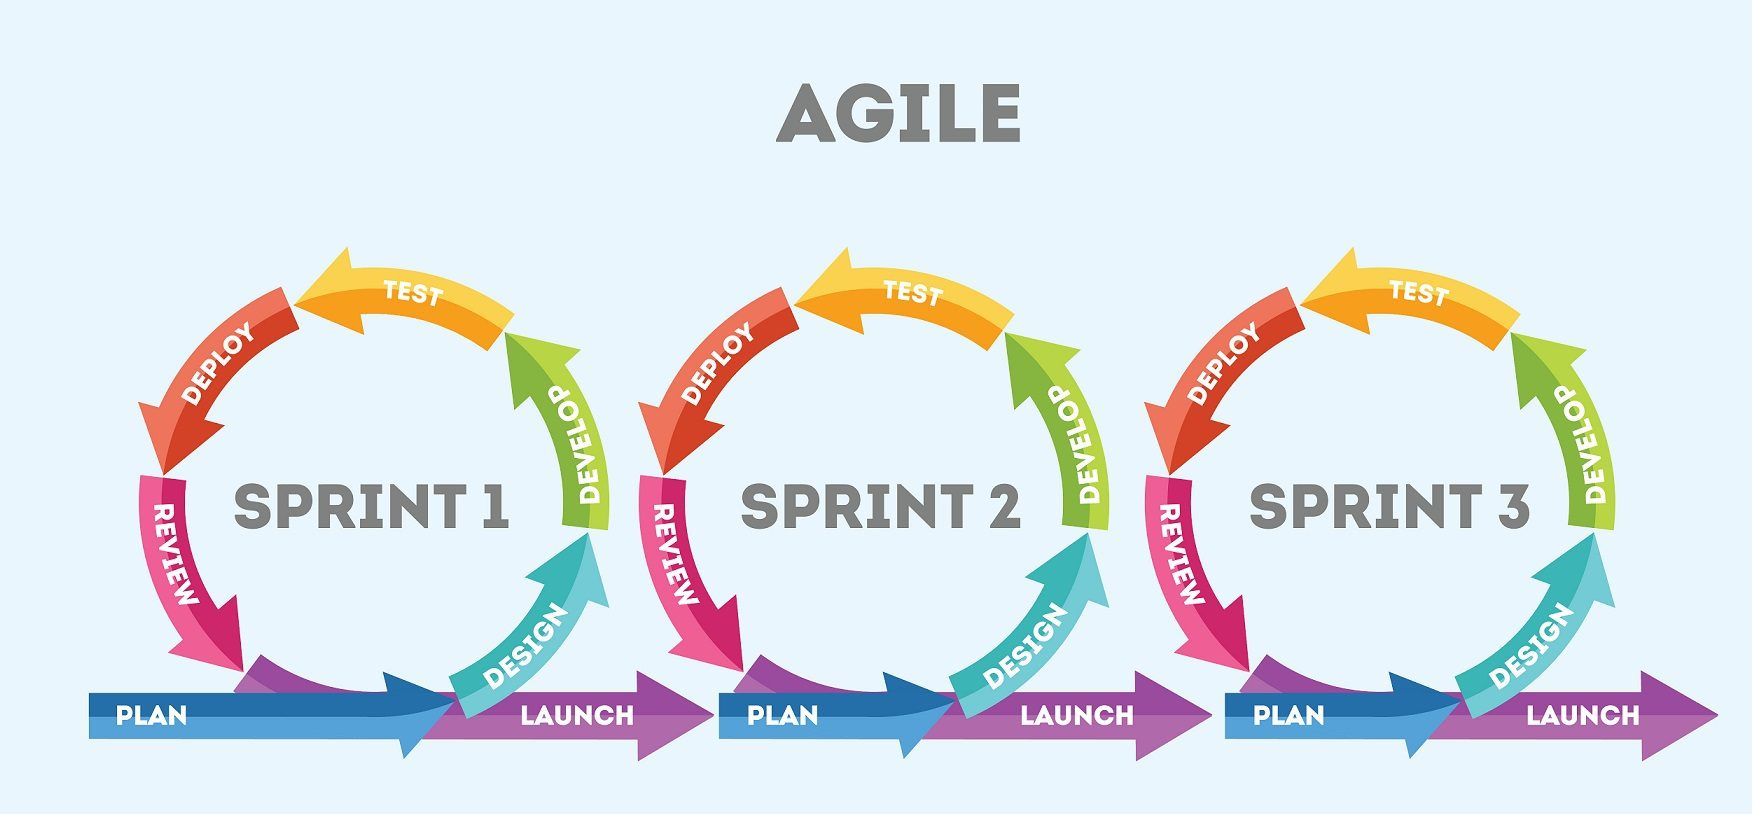
\includegraphics[width=0.8\textwidth]{image/Background/Agile-software.jpeg}
      \caption[Agile]{Agile concept}
      \label{fig:agile_pic}
    \end{figure}
    \FloatBarrier
    \qquad Agile เป็นแนวทางการพัฒนาซอฟต์แวร์ที่เน้นการทำงานร่วมกันอย่างใกล้ชิดระหว่างทีมพัฒนาและผู้มีส่วนได้ส่วนเสีย
    โดยมีการแบ่งงานออกเป็นรอบสั้น ๆ ที่เรียกว่า สปรินต์ (Sprints) ซึ่งแต่ละสปรินต์จะมีการวางแผน การพัฒนา และการทดสอบอย่างรวดเร็ว
    Agile เน้นการตอบสนองต่อการเปลี่ยนแปลงอย่างรวดเร็ว และการส่งมอบซอฟต์แวร์ที่มีคุณภาพสูงอย่างต่อเนื่อง โดยมีหลักการสำคัญดังนี้ \cite{Agile}
    \begin{enumerate}
      \item การทำงานร่วมกันระหว่างทีมพัฒนาและผู้มีส่วนได้ส่วนเสียอย่างใกล้ชิด
      \item การแบ่งงานออกเป็นรอบสั้น ๆ ที่เรียกว่า สปรินต์ (Sprints)
      \item การตอบสนองต่อการเปลี่ยนแปลงอย่างรวดเร็ว
      \item การส่งมอบซอฟต์แวร์ที่มีคุณภาพสูงอย่างต่อเนื่อง
      \item การปรับปรุงกระบวนการพัฒนาอย่างต่อเนื่อง
      \item การให้ความสำคัญกับบุคคลและปฏิสัมพันธ์มากกว่ากระบวนการและเครื่องมือ
    \end{enumerate}
  \subsection{REST API}
    \begin{figure}[!h]
      \centering
      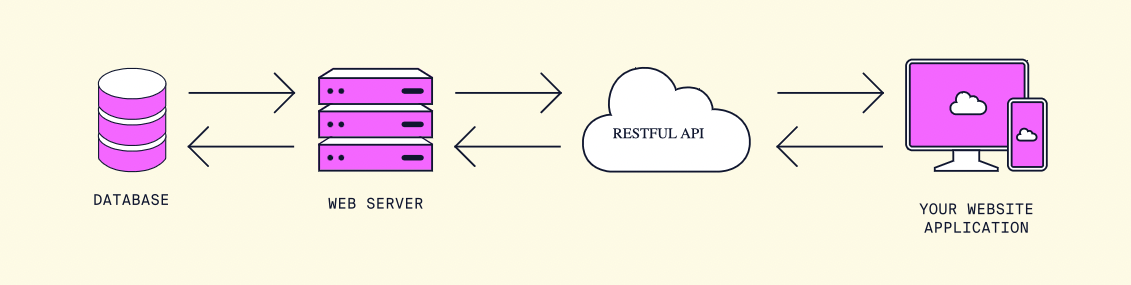
\includegraphics[width=0.8\textwidth]{image/Background/REST-API.png}
      \caption[REST API]{REST API concept}
      \label{fig:api_pic}
    \end{figure}
    \qquad REST ย่อมาจาก Representational State Transfer เป็นรูปแบบการส่งข้อมูลระหว่าง Server Client
    รูปแบบหนึ่งซึ่งอยู่บนพื้นฐานของ HTTP Protocol เป็นการสร้าง Web Service เพื่อแลกเปลี่ยน ข้อมูลกันผ่าน Application
    วิธีหนึ่งซึ่งส่งข้อมูลได้หลายชนิด ไม่ว่าจะเป็น Text, XML, JSON หรือแม้แต่ HTML ก็สามารถส่งได้ \cite{API}
    
    \qquad API ย่อมาจาก Application Programming Interface คือการเชื่อมต่อจากระบบหนึ่งไปยังอีกระบบหนึ่งเพื่อให้ซอฟต์แวร์
    ภายนอกเข้าถึงและอัพเดทข้อมูลนั้นๆได้ แต่ยังอยู่ภายในขอบเขตที่ถูกกําหนดไว้ กล่าวคือ API เป็นตัวกลางที่จะทําให้คอยรับคําสั่งต่างๆ 
    ประมวลผลและกระทําข้อมูลส่งกลับคืนไปยังคนสั่งโดยอัตโนมัติ \cite{RESTAPI}
  \subsection{Hexagonal Architecture}
    \begin{figure}[!h]
      \centering
      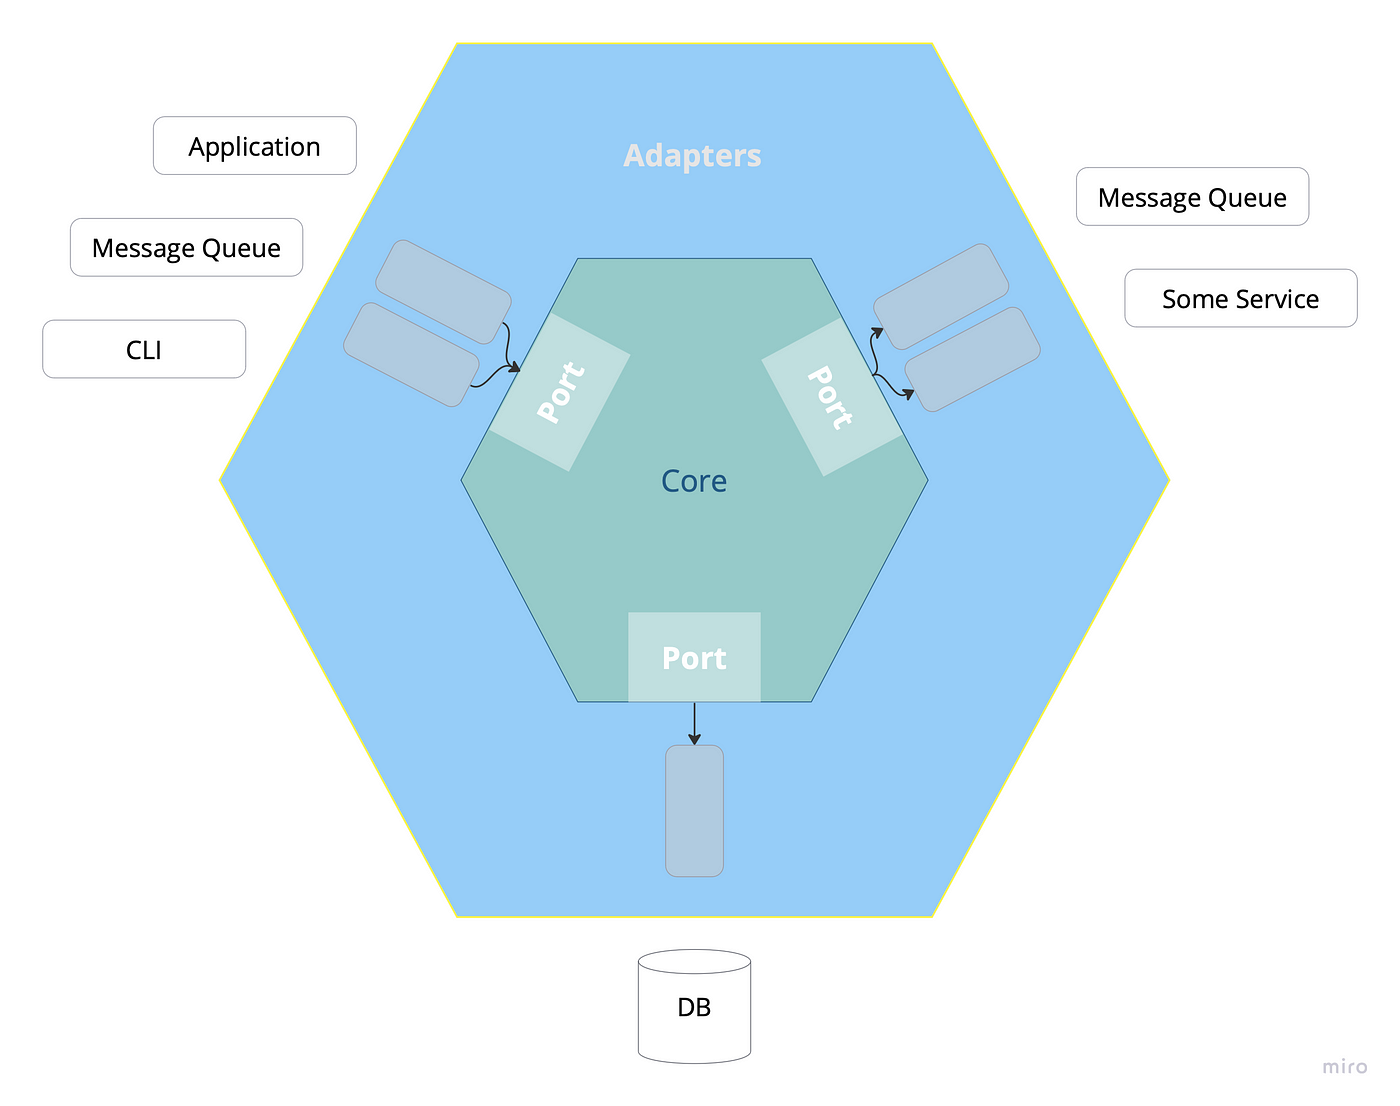
\includegraphics[width=0.6\textwidth]{image/Background/hex.png}
      \caption[Hexagonal Architecture]{โครงสร้างสถาปัตยกรรม Hexagonal}
      \label{fig:hex_pic}
    \end{figure}
    \FloatBarrier
    \qquad Hexagonal Architecture เป็น 1 ใน Code Architecture Pattern ที่เป็นที่นิยมของ Go ที่สร้างอยู่บน 2 pattern หลักๆ คือ Adaptor Pattern และ Dependency Injection  โดยองค์ประกอบหลักของ Hexagonal Architecture จะประกอบด้วยของ 3 อย่าง \cite{Hexagonal1}\cite{Hexagonal2}
    \begin{enumerate}
      \item Ports: เป็นส่วนของ Interfaces ที่กำหนดวิธีการที่แอปพลิเคชันสามารถเชื่อมต่อและติดต่อสื่อสารกับส่วนของ business logic รวมถึงการเข้าถึงทรัพยากรภายนอก โดย Ports ทำหน้าที่เป็นประตูการเชื่อมต่อระหว่าง business logic และระบบภายนอก ทำให้การเชื่อมโยงข้อมูลหรือบริการเป็นไปตามรูปแบบที่กำหนด\
      \item Adapters: เป็นส่วนที่ทำหน้าที่เชื่อมต่อกับ Ports เปรียบเสมือน "สะพาน" ที่เชื่อมโยงระหว่างทรัพยากรภายนอกจริง (เช่น ฐานข้อมูล, บริการเว็บเซอร์วิส) กับ business logic โดย Adapters จะทำหน้าที่แปลงข้อมูลระหว่าง Ports กับทรัพยากรที่ติดต่อด้วย เพื่อให้การสื่อสารระหว่าง business logic และระบบภายนอกสามารถทำงานร่วมกันได้อย่างราบรื่น
      \item Domain-centric เป็นส่วนที่อยู่ตรงกลางของ business logic และเป็นศูนย์กลางของการประมวลผลและการคำนวณต่างๆ ในแอปพลิเคชัน ทำหน้าที่จัดการตรรกะหลักของระบบโดยไม่ผูกติดกับการทำงานของระบบภายนอก เป็นศูนย์กลางของกระบวนการและกฎทางธุรกิจ (business rules) เพื่อให้ระบบมีความเป็นอิสระและแยกจากการพึ่งพาทรัพยากรภายนอก
    \end{enumerate}
    \subsection{Reverse Proxy}
    \begin{figure}[!h]
      \centering
      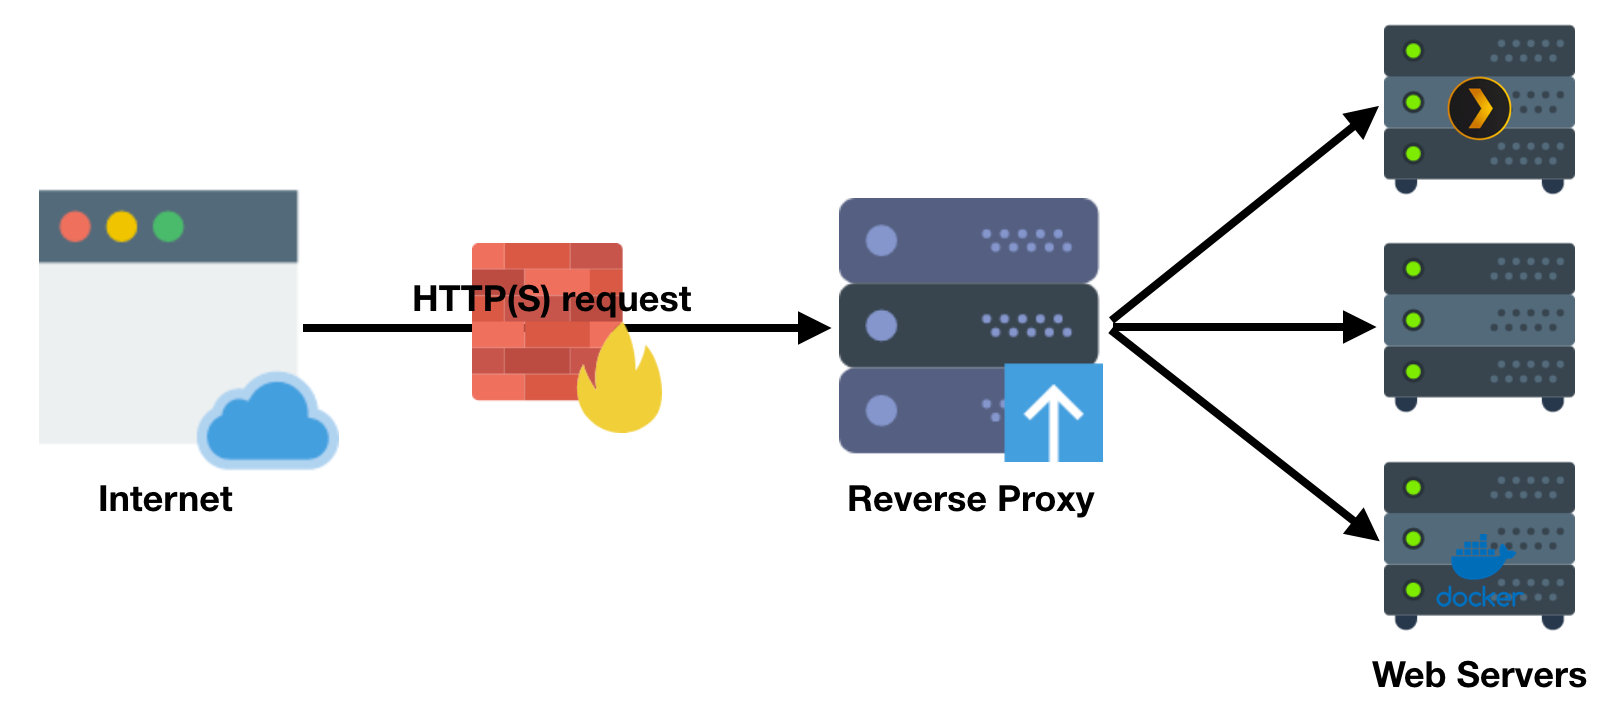
\includegraphics[width=0.6\textwidth]{image/Background/Reverse-proxy.png}
      \caption[Reverse Proxy]{Structure of Reverse Proxy}
      \label{fig:reverse_proxy_pic}
    \end{figure}
    \qquad Reverse Proxy คือ เซิร์ฟเวอร์ที่ทำหน้าที่เป็นตัวกลางระหว่างผู้ใช้ (Clients) กับเซิร์ฟเวอร์หลัก (Origin Servers)
    โดย Reverse Proxy จะรับคำขอ (Requests) จากผู้ใช้และส่งต่อไปยังเซิร์ฟเวอร์หลัก จากนั้นจะรับคำตอบ (Responses)
    จากเซิร์ฟเวอร์หลักและส่งกลับไปยังผู้ใช้ อีกครั้ง Reverse Proxy มีประโยชน์หลายประการ เช่น \cite{ReverseProxy}
    \begin{enumerate}
      \item การเพิ่มประสิทธิภาพ: Reverse Proxy สามารถทำหน้าที่เป็นตัวเก็บแคช (Cache) เพื่อเก็บข้อมูลที่ถูกเรียกใช้งานบ่อยๆ
      ซึ่งช่วยลดภาระงานของเซิร์ฟเวอร์หลักและเพิ่มความเร็วในการตอบสนองต่อผู้ใช้
      \item การกระจายโหลด: Reverse Proxy สามารถกระจายคำขอไปยังเซิร์ฟเวอร์หลักหลายๆ ตัว
      ซึ่งช่วยให้ระบบสามารถรองรับการใช้งานที่มีปริมาณมากได้อย่างมีประสิทธิภาพ
      \item ความปลอดภัย: Reverse Proxy สามารถทำหน้าที่เป็นเกราะป้องกัน (Firewall)
      โดยการกรองคำขอที่ไม่ปลอดภัยและป้องกันการโจมตีจากภายนอก
      \item การจัดการ SSL/TLS: Reverse Proxy สามารถจัดการการเข้ารหัสข้อมูลด้วย SSL/TLS
      แทนเซิร์ฟเวอร์หลัก ซึ่งช่วยลดภาระงานของเซิร์ฟเวอร์หลักและทำให้การจัดการใบรับรองดิจิทัลง่ายขึ้น
    \end{enumerate}
    
  \subsection{Tailwind CSS}
    \qquad ข้างบนเป็นรูป ตรงนี้เป็นคำอธิบาย อย่าลืมใส่แหล่งอ้างอิง \cite{Tailwind}
  \subsection{MantineUI}
    \qquad ข้างบนเป็นรูป ตรงนี้เป็นคำอธิบาย อย่าลืมใส่แหล่งอ้างอิง \cite{Mantine}

  \subsection{App Router}
    \begin{figure}[!h]
      \centering
      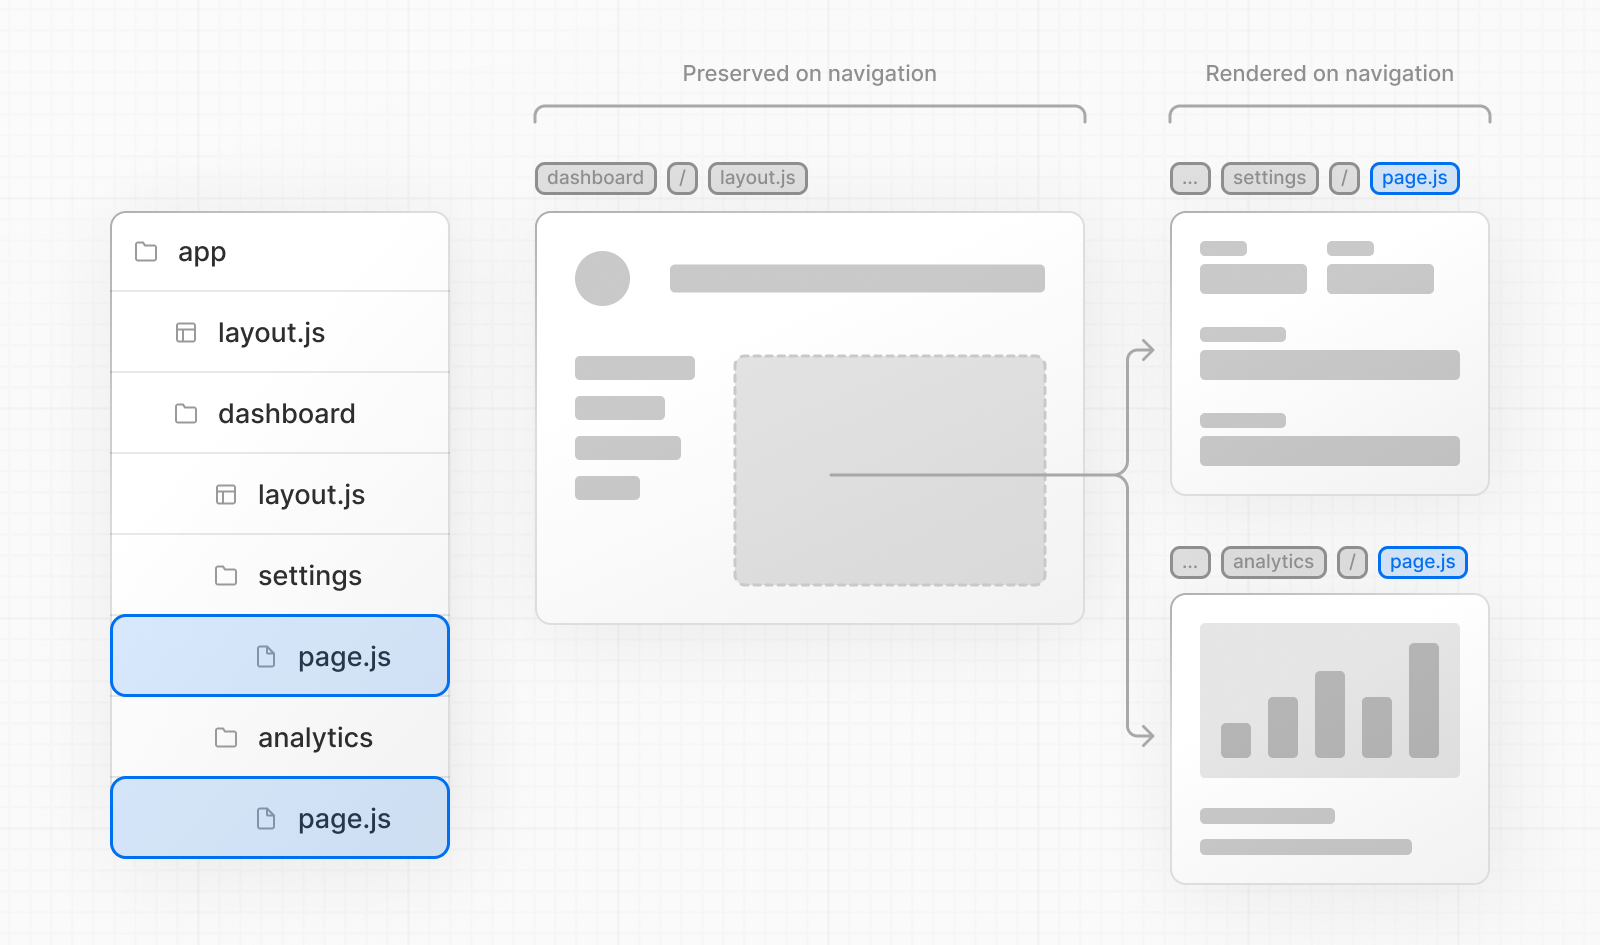
\includegraphics[width=0.6\textwidth]{image/Background/app-router.png}
      \caption[App Router]{โครงสร้างของ App Router}
      \label{fig:app_router_pic}
    \end{figure}
    \FloatBarrier
    \qquad App Router เป็นเครื่องมือที่ช่วยในการจัดการเส้นทาง (Routing) ของแอปพลิเคชันเว็บ
    ซึ่งช่วยให้การนำทางระหว่างหน้าและส่วนต่างๆ ของแอปพลิเคชันเป็นไปอย่างราบรื่นและมีประสิทธิภาพ โดย App Router
    จะทำหน้าที่จับคู่ URL ที่ผู้ใช้ร้องขอเข้ากับคอมโพเนนต์หรือหน้าที่เหมาะสมในแอปพลิเคชัน ซึ่งช่วยให้ผู้พัฒนาสามารถสร้างแอปพลิเคชัน
    ที่มีโครงสร้างที่ชัดเจนและง่ายต่อการดูแลรักษา นอกจากนี้ App Router ยังสนับสนุนฟีเจอร์ต่างๆ เช่น การจัดการสถานะของหน้า
    การส่งผ่านพารามิเตอร์ และการจัดการเส้นทางแบบไดนามิก ทำให้ผู้ใช้สามารถเข้าถึงเนื้อหาต่างๆ ได้อย่างรวดเร็วและสะดวกสบาย
    \cite{AppRouter} \cite{Routing}

  \subsection{Json Web Token (JWT)}
    \begin{figure}[!h]
      \centering
      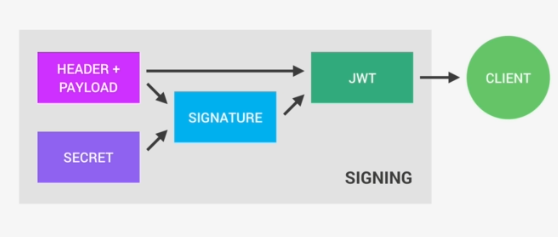
\includegraphics[width=0.6\textwidth]{image/Background/JWT.png}
      \caption[JWT]{โครงสร้างของ Json Web Token (JWT)}
      \label{fig:jwt_pic}
    \end{figure}
    \FloatBarrier
    \qquad JWT[?]เป็นมาตรฐานแบบเปิด (RFC 7519) ที่กําหนดรูปแบบข้อมูลที่มีขนาดเล็กและสามารถตรวจสอบได้ในตัวเอง
    เพื่อใช้ในการส่งข้อมูลระหว่างฝ่ายต่างๆ อย่างปลอดภัยในรูปแบบของ JSON ข้อมูลนี้สามารถตรวจสอบและเชื่อถือได้
    เนื่องจากมีการลงนามดิจิทัล (Digitally signed) \cite{JWT}

\section{Database System}
  \qquad ระบบฐานข้อมูล (Database System) หมายถึงโครงสร้างสารสนเทศที่ประกอบด้วย รายละเอียดของข้อมูลที่เกี่ยวข้องกัน
  ที่จะนำมาใช้ในระบบต่างๆ ร่วมกัน ซึ่งผู้ใช้สามารถจัดการกับ ข้อมูลได้ในลักษณะต่างๆ ทั้งเพิ่ม ลบ หรือแก้ไข
  ตลอดจนการเรียกดูข้อมูลส่วนใหญ่จะเป็นการประยุกต์นำเอาระบบคอมพิวเตอร์เข้ามาช่วยในการจัดการฐานข้อมูลระบบฐานข้อมูล
  มีคําศัพท์ต่างๆที่เกี่ยวข้องดังนี้ \cite{DataBaseSystem}
  \subsection{Entity}
    \qquad Entity คือ สิ่งที่สามารถระบุได้อย่างชัดเจน เช่น บุคคล สถานที่ สิ่งของ เหตุการณ์ หรือแนวคิด ซึ่งมีความสำคัญในบริบท
    ของระบบฐานข้อมูล โดย Entity จะถูกแทนด้วยตาราง (Table) ในฐานข้อมูล และแต่ละแถว (Row) ในตารางจะเป็นการแสดงถึง
    ตัวอย่างเฉพาะของ Entity นั้นๆ เช่น ในระบบฐานข้อมูลของมหาวิทยาลัย "นักศึกษา" อาจเป็น Entity หนึ่ง โดยแต่ละแถว
    ในตารางนักศึกษาจะเป็นการแสดงถึงนักศึกษาแต่ละคนที่มีข้อมูลเฉพาะตัว เช่น ชื่อ รหัสนักศึกษา และวันเกิด \cite{Entity}
  \subsection{Attribute}
    \qquad Attribute คือ คุณสมบัติหรือลักษณะเฉพาะของ Entity ที่ใช้ในการอธิบายหรือระบุข้อมูลเพิ่มเติมเกี่ยวกับ Entity นั้นๆ
    ในระบบฐานข้อมูล Attribute จะถูกแทนด้วยคอลัมน์ (Column) ในตาราง และแต่ละคอลัมน์จะเก็บข้อมูลเฉพาะเจาะจงเกี่ยวกับ
    Entity ตัวอย่างเช่น ในตารางนักศึกษา Attribute อาจประกอบด้วย ชื่อ (name), รหัสนักศึกษา (student ID),
    วันเกิด (date of birth) เป็นต้น ซึ่งแต่ละ Attribute จะมีค่าที่แตกต่างกันสำหรับแต่ละแถวในตาราง \cite{Attribute}
  \subsection{Relationship}
    \qquad Relationship คือ ความสัมพันธ์ระหว่าง Entity ต่างๆ ในระบบฐานข้อมูล ซึ่งแสดงถึงวิธีที่ Entity เหล่านั้นเชื่อมโยง
    หรือมีปฏิสัมพันธ์กัน โดย Relationship จะถูกแทนด้วยตารางความสัมพันธ์ (Relationship table)
    หรือคอลัมน์ในตารางที่เชื่อมโยง Entity ต่าง ๆ เข้าด้วยกัน ตัวอย่างเช่น ในระบบฐานข้อมูลของมหาวิทยาลัย อาจมี
    Relationship ระหว่าง Entity "นักศึกษา" กับ "หลักสูตร" ที่แสดงว่านักศึกษาแต่ละคนสามารถลงทะเบียนเรียนในหลักสูตรต่างๆ ได้อย่างไร
  \subsection{Primary Key}
    \qquad Primary Key คือ คอลัมน์หรือชุดของคอลัมน์ในตารางฐานข้อมูลที่มีคุณสมบัติพิเศษที่ใช้ในการระบุแถว (Row)
    แต่ละแถวในตารางอย่างไม่ซ้ำกัน Primary Key จะต้องมีค่าที่ไม่ซ้ำกัน (Unique) และไม่เป็นค่า null (Not null)
    ในแต่ละแถวของตาราง ซึ่งช่วยให้สามารถเข้าถึงและจัดการข้อมูลได้อย่างมีประสิทธิภาพ นอกจากนี้ Primary Key
    ยังช่วยในการสร้างความสัมพันธ์ระหว่างตารางต่างๆ ในฐานข้อมูลผ่านการใช้คีย์นอก (Foreign key) ที่เชื่อมโยงกับ
    Primary Key ของตารางอื่นๆ \cite{PrimaryKey}
  \subsection{Foreign Key}
    \qquad Foreign Key คือ คอลัมน์หรือชุดของคอลัมน์ในตารางฐานข้อมูลที่ใช้เพื่อสร้างความสัมพันธ์ระหว่างตารางต่างๆ โดย
    Foreign Key จะอ้างอิงถึง Primary Key ของตารางอื่น ซึ่งช่วยให้สามารถเชื่อมโยงข้อมูลระหว่างตารางได้อย่างมีประสิทธิภาพ
    Foreign Key ช่วยในการรักษาความสมบูรณ์ของข้อมูล (Data integrity) โดยการบังคับใช้ข้อจำกัดที่ทำให้ค่าของ
    Foreign Key ต้องตรงกับค่าของ Primary Key ในตารางที่อ้างอิง หรือเป็นค่า Null เท่านั้น \cite{ForeignKey}
  \subsection{Relational Database Management System (RDBMS)}
    \qquad RDBMS เป็นระบบจัดการฐานข้อมูลที่ใช้โครงสร้างแบบตาราง (table) เพื่อจัดเก็บข้อมูล โดยแต่ละตารางจะประกอบด้วย
    แถว (Row) และคอลัมน์ (Column) ซึ่งช่วยให้การจัดการและการเข้าถึงข้อมูลเป็นไปอย่างมีประสิทธิภาพ RDBMS ใช้ภาษา SQL
    (Structured Query Language) ในการสร้าง แก้ไข และดึงข้อมูลจากฐานข้อมูล นอกจากนี้ RDBMS ยังสนับสนุนความสัมพันธ์
    ระหว่างตารางต่างๆ ผ่านคีย์หลัก (Primary Key) และคีย์นอก (Foreign Key) ซึ่งช่วยให้สามารถเชื่อมโยงข้อมูลระหว่างตาราง
    ได้อย่างมีประสิทธิภาพ \cite{RDBMS}

\section{Storage}
  \subsection{Object Storage}
    \qquad Object Storage คือ รูปแบบการจัดเก็บข้อมูลที่ใช้ในการจัดการและเก็บข้อมูลในรูปแบบของวัตถุ (Objects)
    ซึ่งแต่ละวัตถุจะประกอบด้วยข้อมูล (Data) และเมตาดาต้า (Metadata) ที่อธิบายลักษณะและคุณสมบัติของข้อมูลนั้นๆ 
    Object Storage มีความยืดหยุ่นสูง สามารถจัดเก็บข้อมูลได้หลากหลายประเภท เช่น ไฟล์ภาพ วิดีโอ เอกสาร และข้อมูลอื่นๆ
    โดยไม่จำเป็นต้องมีโครงสร้างตารางเหมือนกับฐานข้อมูลแบบดั้งเดิม นอกจากนี้ Object Storage ยังมีความสามารถในการขยายตัว
    (Scalability) ที่ดี ทำให้สามารถรองรับปริมาณข้อมูลที่เพิ่มขึ้นได้อย่างมีประสิทธิภาพ \cite{ObjectStorage}
  \subsection{Metadata}
    \qquad Metadata คือ ข้อมูลที่อธิบายลักษณะและคุณสมบัติของข้อมูลอื่นๆ ซึ่งช่วยให้สามารถจัดการ ค้นหา และใช้งานข้อมูล
    ได้อย่างมีประสิทธิภาพ \cite{Metadata}
  \subsection{Bucket}
    \qquad Bucket คือ โครงสร้างหลักที่ใช้ในการจัดเก็บข้อมูลไฟล์ต่างๆ ในระบบจัดเก็บข้อมูลแบบอ็อบเจ็กต์ โดย Bucket
    ทำหน้าที่เป็นที่เก็บข้อมูลที่มีการจัดระเบียบและแยกประเภทอย่างชัดเจน ซึ่งช่วยให้การจัดการและการเข้าถึงข้อมูลเป็นไปอย่าง
    มีประสิทธิภาพ ในแต่ละ Bucket สามารถเก็บวัตถุ (Objects) ได้หลากหลายประเภท เช่น ไฟล์ภาพ วิดีโอ เอกสาร
    และข้อมูลอื่นๆ นอกจากนี้ Bucket ยังสามารถกำหนดสิทธิ์การเข้าถึงข้อมูลได้อย่างละเอียด เพื่อควบคุมการใช้งานและ
    รักษาความปลอดภัยของข้อมูล \cite{Bucket}

\section{Optical Character Recognition (OCR)}
  \qquad Optical Character Recognition (OCR) คือ เทคโนโลยีที่ใช้ในการแปลงภาพตัวอักษรที่ถูกสแกนหรือ
  ถ่ายภาพมาให้อยู่ในรูปแบบดิจิทัลที่สามารถแก้ไขและค้นหาได้ OCR ทำงานโดยการวิเคราะห์ภาพเพื่อระบุและแยกแยะตัวอักษร
  จากนั้นจึงแปลงตัวอักษรเหล่านั้นเป็นข้อความที่สามารถนำไปใช้ในโปรแกรมประมวลผลคำหรือฐานข้อมูลได้ 
  เทคโนโลยี OCR มีการใช้งานอย่างแพร่หลายในหลายๆ ด้าน เช่น การแปลงเอกสารกระดาษเป็นไฟล์ดิจิทัล 
  การสแกนบัตรประชาชน หรือการอ่านป้ายทะเบียนรถยนต์ เป็นต้น \cite{OCR}
  \subsection{Tesseract OCR}
    \qquad Tesseract OCR เป็นซอฟต์แวร์โอเพนซอร์สที่ใช้สำหรับการรู้จำอักขระด้วยแสง 
    (Optical Character Recognition - OCR) ซึ่งพัฒนาโดย Google Tesseract
    มีความสามารถในการแปลงภาพของตัวอักษรที่ถูกสแกนหรือถ่ายภาพมาให้อยู่ในรูปแบบดิจิทัลที่สามารถแก้ไขและค้นหาได้
    ซอฟต์แวร์นี้รองรับหลายภาษาและสามารถทำงานกับรูปแบบภาพต่างๆ เช่น JPEG, PNG, TIFF เป็นต้น Tesseract OCR
    มีการใช้งานอย่างแพร่หลายในหลายๆ ด้าน เช่น การแปลงเอกสารกระดาษเป็นไฟล์ดิจิทัล การสแกนบัตรประชาชน
    หรือการอ่านป้ายทะเบียนรถยนต์ เป็นต้น โดยข้อดีของ Tesseract OCR มีดังนี้ \cite{Tesseract}
    \begin{enumerate}
      \item เป็นซอฟต์แวร์โอเพนซอร์สที่สามารถใช้งานได้ฟรี
      \item รองรับหลายภาษาและรูปแบบภาพต่างๆ
      \item มีความแม่นยำในการรู้จำอักขระสูง
      \item สามารถปรับแต่งและขยายความสามารถได้ตามความต้องการของผู้ใช้
    \end{enumerate}

\section{Third section}
Section 3 text. The dielectric constant\index{dielectric constant}
at the air-metal interface determines
the resonance shift\index{resonance shift} as absorption or capture occurs
is shown in Equation~\eqref{eq:dielectric}:

\begin{equation}\label{eq:dielectric}
k_1=\frac{\omega}{c({1/\varepsilon_m + 1/\varepsilon_i})^{1/2}}=k_2=\frac{\omega
\sin(\theta)\varepsilon_\mathit{air}^{1/2}}{c}
\end{equation}

\noindent
where $\omega$ is the frequency of the plasmon, $c$ is the speed of
light, $\varepsilon_m$ is the dielectric constant of the metal,
$\varepsilon_i$ is the dielectric constant of neighboring insulator,
and $\varepsilon_\mathit{air}$ is the dielectric constant of air.

\section{About using figures in your report}

% define a command that produces some filler text, the lorem ipsum.
\newcommand{\loremipsum}{
  \textit{Lorem ipsum dolor sit amet, consectetur adipisicing elit, sed do
  eiusmod tempor incididunt ut labore et dolore magna aliqua. Ut enim ad
  minim veniam, quis nostrud exercitation ullamco laboris nisi ut
  aliquip ex ea commodo consequat. Duis aute irure dolor in
  reprehenderit in voluptate velit esse cillum dolore eu fugiat nulla
  pariatur. Excepteur sint occaecat cupidatat non proident, sunt in
  culpa qui officia deserunt mollit anim id est laborum.}\par}

\begin{figure}
  \centering

  \fbox{
     \parbox{.6\textwidth}{\loremipsum}
  }

  % To include an image in the figure, say myimage.pdf, you could use
  % the following code. Look up the documentation for the package
  % graphicx for more information.
  % \includegraphics[width=\textwidth]{myimage}

  \caption[Sample figure]{This figure is a sample containing \gls{lorem ipsum},
  showing you how you can include figures and glossary in your report.
  You can specify a shorter caption that will appear in the List of Figures.}
  \label{fig:sample-figure}
\end{figure}

Using \verb.\label. and \verb.\ref. commands allows us to refer to
figures easily. If we can refer to Figures
\ref{fig:walrus} and \ref{fig:sample-figure} by name in the {\LaTeX}
source code, then we will not need to update the code that refers to it
even if the placement or ordering of the figures changes.

\loremipsum\loremipsum

% This code demonstrates how to get a landscape table or figure. It
% uses the package lscape to turn everything but the page number into
% landscape orientation. Everything should be included within an
% \afterpage{ .... } to avoid causing a page break too early.
\afterpage{
  \begin{landscape}
  \begin{table}
    \caption{Sample landscape table}
    \label{tab:sample-table}

    \centering

    \begin{tabular}{c||c|c}
        Year & A & B \\
        \hline\hline
        1989 & 12 & 23 \\
        1990 & 4 & 9 \\
        1991 & 3 & 6 \\
    \end{tabular}
  \end{table}
  \end{landscape}
}

\loremipsum\loremipsum\loremipsum

\section{Overfull hbox}

When the \verb.semifinal. option is passed to the \verb.cpecmu. document class,
any line that is longer than the line width, i.e., an overfull hbox, will be
highlighted with a black solid rule:
\begin{center}
\begin{minipage}{2em}
juxtaposition
\end{minipage}
\end{center}

\section{\ifenglish%
\ifcpe CPE \else ISNE \fi knowledge used, applied, or integrated in this project
\else%
ความรู้ตามหลักสูตรซึ่งถูกนำมาใช้หรือบูรณาการในโครงงาน
\fi
}

อธิบายถึงความรู้ และแนวทางการนำความรู้ต่างๆ ที่ได้เรียนตามหลักสูตร ซึ่งถูกนำมาใช้ในโครงงาน

\section{\ifenglish%
Extracurricular knowledge used, applied, or integrated in this project
\else%
ความรู้นอกหลักสูตรซึ่งถูกนำมาใช้หรือบูรณาการในโครงงาน
\fi
}

อธิบายถึงความรู้ต่างๆ ที่เรียนรู้ด้วยตนเอง และแนวทางการนำความรู้เหล่านั้นมาใช้ในโครงงาน
